\section{Interfaces}
\subsection{Web Interface}
\index{Web Interface}
The main interface for the PLM is provided by a web application.  The web 
application allows users to add/delete their own patches as well as view 
information on patches already in the database.  A search interface is also 
available.

\subsubsection{Home Page}
\index{Web Interface!Home Page}
The home page provides some basic information about the PLM and provides links to
HOWTO information.  The user navigates to the rest of the main pages through the 
buttons on the top navigation bar.

\begin{center}
\scalebox{0.75}{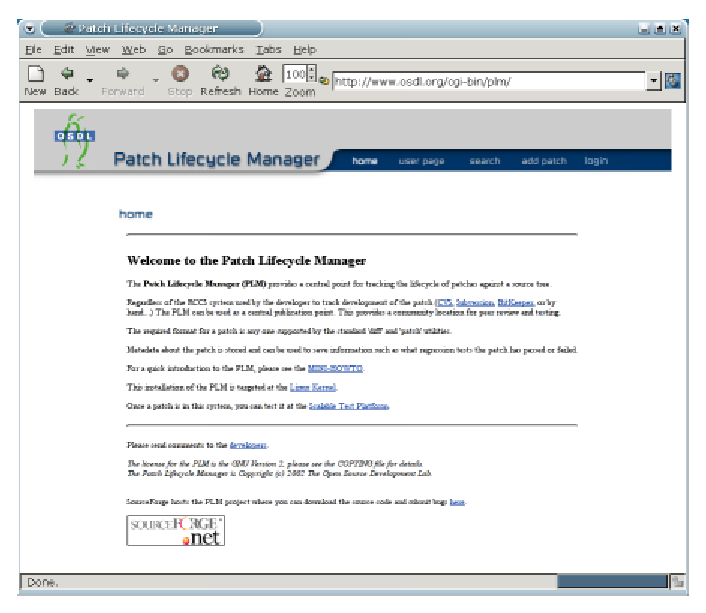
\includegraphics{images/home_page.ps}}
\end{center}

\subsubsection{User Page}
\index{Web Interface!User Page}
The user page provides a quick activity summary for an authenticated user.
Information provided includes the users login name, email address and a search 
report on the most recent patches submitted by the user.

\begin{center}
\scalebox{0.75}{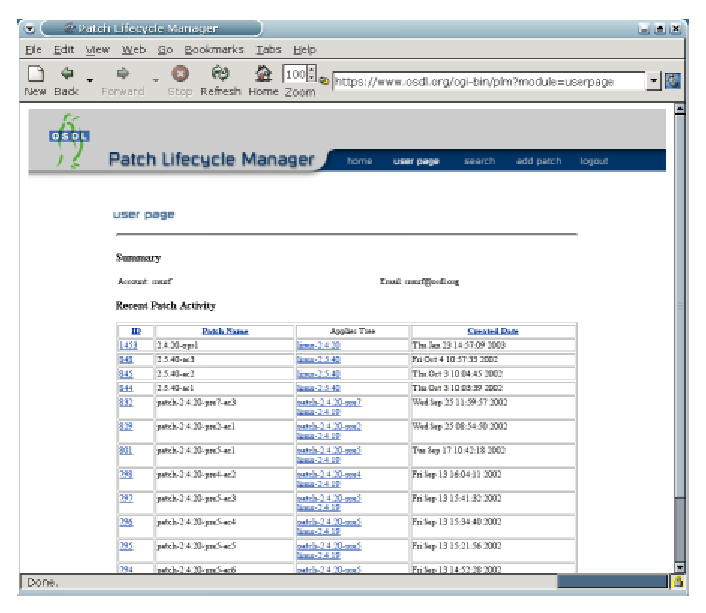
\includegraphics{images/user_page.ps}}
\end{center}

\subsubsection{Search Page}
\index{Web Interface!Search Page}
The search page provides an easy interface for finding both base software 
versions and patches.  The potential search parameters are:

\begin{itemize}
\item Patch \emph{name} or \emph{ID}
\item Name of the submitter
\item Creation date (selection from a drop-down box of possible values)
\end{itemize}

\begin{center}
\scalebox{0.75}{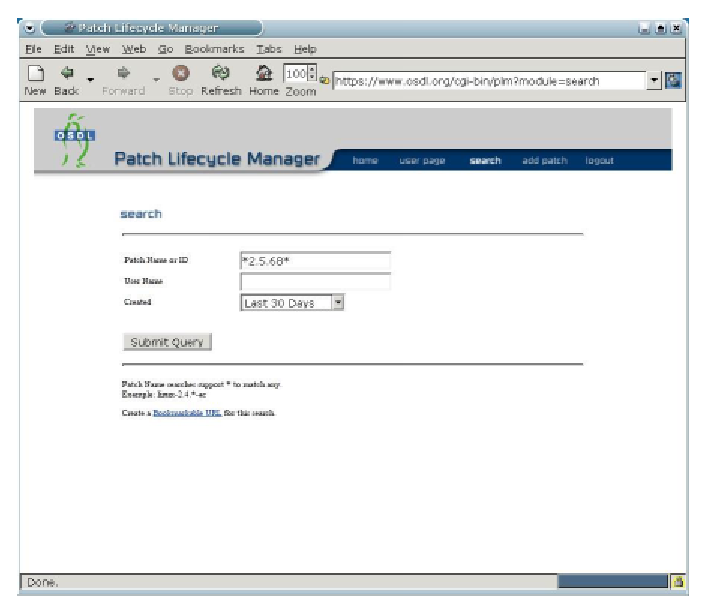
\includegraphics{images/search_page.ps}}
\end{center}

The results of the search will have hyperlinks to the \emph{Patch Information
Page} of each patch listed as well as the patches in their respective applies 
tree.

\begin{center}
\scalebox{0.75}{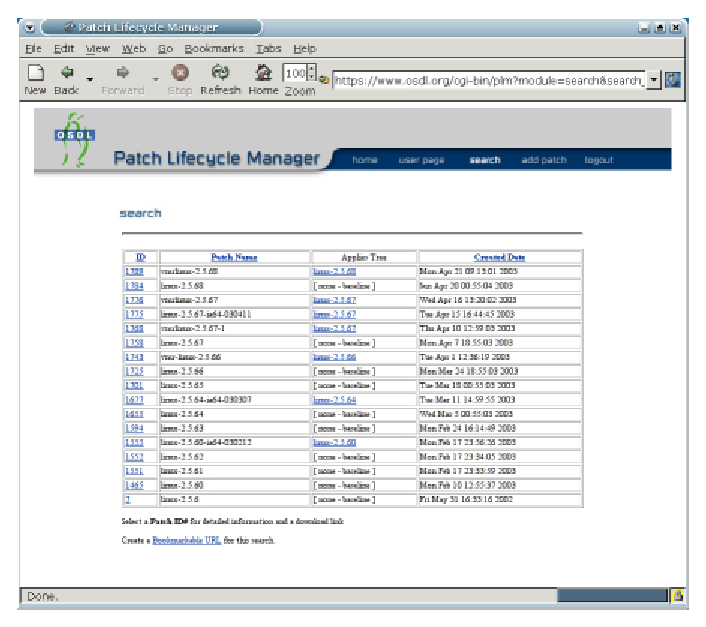
\includegraphics{images/search_results_page.ps}}
\end{center}

\subsubsection{Login Page}
\index{Web Interface!Login}
Anytime you either select the login button on the top menu, or select a page that 
requires a login, you will be prompted for your username and password.

\begin{center}
\scalebox{0.75}{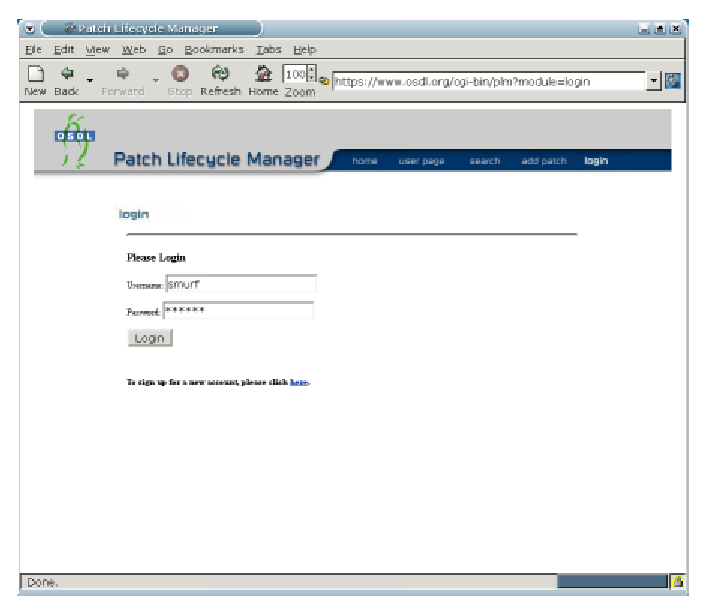
\includegraphics{images/login_page.ps}}
\end{center}

\subsubsection{Add Patch Page}
\index{Web Interface!Add Patch}
The add patch page provides a quick interface for adding new patches into the
system.  The user is required to provide the following information:

\begin{itemize}
\item Name of patch
\item Name or ID of patch to apply to
\item Content (provided by file-upload)
\end{itemize}

\begin{center}
\scalebox{0.75}{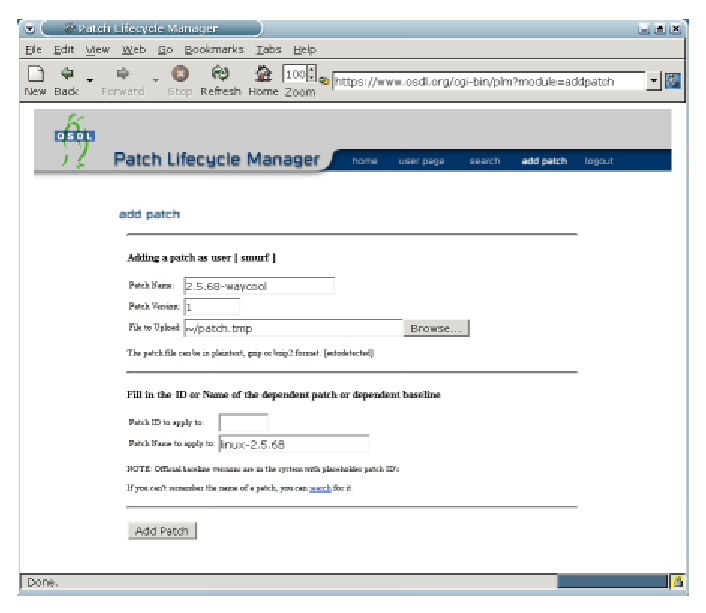
\includegraphics{images/add_patch_page.ps}}
\end{center}

The PLM system has a single namespace.  That namespace may have regions 
protected for submission by specified users.  If your patch name steps on one
of these protected regions, you will be notified.  These regions are usually
used to protect official version names.

\subsubsection{Patch Information Page}
\index{Web Interface!Patch Information Page}
The patch information page provides a detailed listing of information regarding
a patch in the PLM system.  

If the version is a base version, a pointer to an external location where the 
user can find the patch is provided.  If the version is a regular patch then 
the user can download the patch from the PLM system.  The user also has the 
options to view the patch in plain text or in code2html output with color 
highlighting.

Information available in the patch information page includes:

\begin{itemize}
\item Original submitter of the patch
\item Submission date \& time
\item The name of the patch
\item md5sum \index{md5sum} of the patch
\item Patch Applies tree with links to relative patch information pages
\item Report on filter results (if available)
\end{itemize}

\begin{center}
\scalebox{0.75}{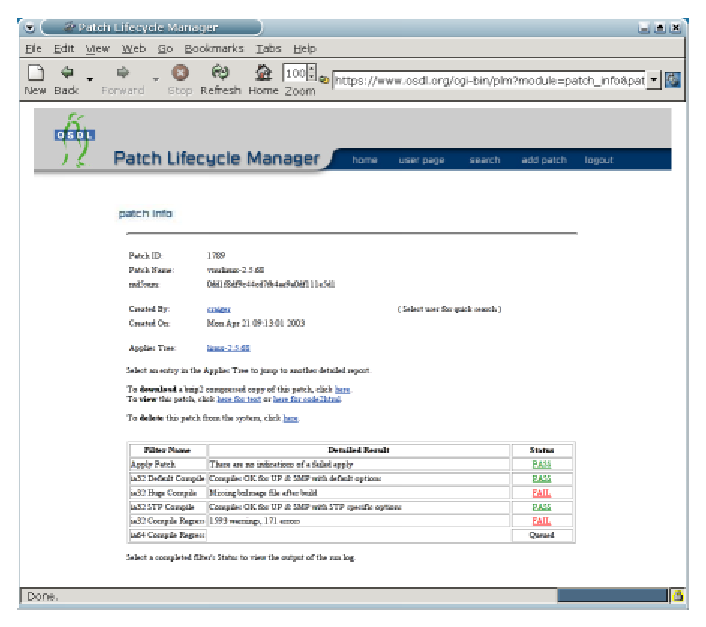
\includegraphics{images/patch_info_page.ps}}
\end{center}

\subsection{Email Interface}
\index{Email Interface}
An email gateway is available with a subset of the web interface's 
functionality. The email gateway can be used by command line scripts for easy 
SCCS=$>$PLM \footnote{The SCCS=$>$PLM gateways will be SCCS specific and have 
not been written yet.} gateway functionality.

The functionality of the email gateway is currently limited to the submission of
new patches.  Patches submitted through the email gateway need to have a limited
amount of meta-data in a special \emph{plm header} to designate parameters such
as the name of the patch and the PLM ID of the baseline or patch that the 
submitted patch applies to.

\subsubsection{Email Gateway Metadata}
\index{Email Interface!Metadata}

If you use the plmsend script, you do NOT NEED to understand this section.

Actions on patches sent in to the PLM are determined by metadata tags included at
the top of the patch in comments. To use a metadata tag, put it at the start of
the patch in the following form: 
	
	\#plm $[$metadata-tag$]$ $[$options...$]$

Each patch has metadata parameters, some are required and some are optional.  
Metadata is included as comments to the patch, for example:

contents of kernel.patch:
\begin{verbatim}
#plm login example-username example-password 
#plm name 2.4.18-rc2 
#plm applies linux-2.4.17
diff -Naur -X /home/marcelo/lib/dontdiff linux.orig/CREDITS linux/CREDITS
\end{verbatim}

The diff line is the start of the actual patch and the \#plm lines will be 
stripped before the patch is saved.

The required lines are:
\begin{itemize}
\item login $[$username$]$ $[$password$]$
\item name "string name for patch"
\item applies "name of the patch or regular version this applies to"
\end{itemize}

Email your patch file (with the metadata included) to the submission address for
the repository you are working with.

You will get an email in response telling you the PLM ID of the accepted patch 
or telling you what went wrong with your submission.  If you don't get any 
email back at all, that means you don't have an account.  We don't respond to 
invalid account emails to avoid being triggered by SPAM.  \footnote{In the future if you 
attempt to login with a '\#plm login' command and your login fails, we will 
email you to let you know.}

Security is obviously an issue when you are sending usernames and passwords
over the Internet.  To keep your information secure, the email interface supports
encryption using the gnupg program available at: http://www.gnu.org/directory/gnuPG.html

\subsection{plmsend script}
\index{Email Interface!plmsend}
'plmsend' is a script for auto-submission of patches.  It will handle the 
encryption and patch metadata information for you.

After downloading the plmsend script, you will want to create a ~/.plmrc file.
The format of this file is as follows:

VARIABLE=VALUE where VARIABLE can be any of:
\begin{itemize}
\item USER - For your username on the PLM system
\item PASS - For your account (make sure the file is readable only by you if
         you include this)
\item PLM\_TO\_ADDR - The email address to submit patches to.  Set this to
PLM\_TO\_ADDR=plm@osdl.org
\end{itemize}
(the following options are optional)

\begin{itemize}
\item ENCRYPT - Encryption is on by default, to disable it, set this to 'off'
\item MAILER - Tell the script to use either 'mail' or 'mutt' to compose the email
\item SANITY - If you don't want to hit enter to confirm a submission, set:
           'SANITY=gone'
\end{itemize}

After you have a valid ~/.plmrc file and have a patch ready, remember you need
to have the following information:

\begin{itemize}
\item Applies - You need to know the patch name that your patch applies to (as
registered in the PLM database).  For regular mainline Linux Kernel
patches, the naming looks /exactly/ like the file on kernel.org
example:  linux-2.4.18  or  patch-2.4.19-pre2
\item Name - Your patch needs a name - include the version in the string.
\item Filename - The name of your file on disk.  If you can't find this, I can't
             help you.
\end{itemize}

Syntax for the plmsend command is:

\begin{verbatim}
plmsend <applies> <name> <filename>
\end{verbatim}

Example plmsend submission command:

\begin{verbatim}
$ plmsend linux-2.4.18 2.4.18-rawio-2 2.4.18-rawio-2.patch
\end{verbatim}
  
\subsection{RPC Interface}
\index{RPC Interface}
There is a limited XML/RPC interface for remote applications.  This interface 
is the one that future command line client scripts will use to interact with 
the main system.

The email gateway is one such remote interface.  It uses the RPC interface as a 
remote back-end for it's library functions.

Authentication is built into the RPC schema to allow the email gateway to run 
in untrusted environments.  There is also a trusted version of the RPC 
interface for environments where security is not an issue.
